\documentclass[10pt,a4paper]{article}
\usepackage[utf8]{inputenc}
\usepackage{tikz}
\usepackage{pgfplots, pgfplotstable}
\usepackage{ae}
\usepackage[brazil]{babel}
\usepackage[vmargin=2cm,hmargin=2cm,columnsep=0.75cm]{geometry}
\usepackage{float,nonfloat}
\usepackage{graphicx,color}
\usepackage{subcaption}
\usepackage{amsmath}
\usepackage{verbatim}
\usepackage{booktabs}
\usepackage{multirow}

\makeatletter
\let\@institution\empty
\def\institution#1{\def\@institution{#1}}
\renewcommand{\maketitle}{
    \begin{center}
        {\Large\bfseries\@title\par\medskip}
        {\large
            \begin{tabular}[t]{c}%
                \@author
        \end{tabular}\par\medskip}
        {\itshape\@institution\par}
        {\itshape\@date\par}
\end{center}}
\makeatother

\newcommand{\pixel}{\textit{pixel} }
\newcommand{\pixels}{\textit{pixels} }
\newcommand{\kernel}{\textit{kernel} }
\newcommand{\kernels}{\textit{kernels} }

\begin{document}
% ============================================================================

\title{MC920: Introdução ao Processamento de Imagem Digital\\Tarefa 8}
\author{
    \begin{minipage}{6cm}
        \centering
        Martin Ichilevici de Oliveira\\
        RA 118077
    \end{minipage}
    \and
    \begin{minipage}{6cm}
        \centering
        Rafael Almeida Erthal Hermano\\
        RA 121286
    \end{minipage}
}
\institution{Instituto de Computação, Universidade Estadual de Campinas}
\date{\today}

\maketitle

% ============================================================================

\section{Critérios de fidelidade aplicados a filtragem de ruídos}
\subsection{Critérios de fidelidade}
\subsubsection{Erro total}
O error total mede o quadrado das diferenças entre os pontos originais e o resultado.

\begin{equation}
    e = \sum_{x = 0}^{M - 1} \sum_{y = 0}^{N - 1} [\hat{f}(x,y) - f(x,y)]^2
    \label{eq:error}
\end{equation}

\subsubsection{Erro médio quadrático}
O erro médio quadrático pode ser definido como:

\begin{equation}
    e_{rms} = \left[\frac{1}{MN} \sum_{x = 0}^{M - 1} \sum_{y = 0}^{N - 1} [\hat{f}(x,y) - f(x,y)]^2 \right]^{\frac{1}{2}}
    \label{eq:error_rms}
\end{equation}

\subsubsection{Relação sinal ruído}
A relação sinal ruído pode ser definida como:

\begin{equation}
    SNR_{ms} =\frac{\sum_{x = 0}^{M - 1} \sum_{y = 0}^{N - 1} \hat{f}(x,y)^{2} }{\sum_{x = 0}^{M - 1} \sum_{y = 0}^{N - 1} [\hat{f}(x,y) - f(x,y)]^2}
    \label{eq:snr}
\end{equation}

\subsection{Critérios de qualidade}
Para imagens cuja finalidade é a observação pelo olho humano, o único método correto de avaliar a qualidade da imagem é a avaliação subjetiva \cite{article}. No campo de processamento de imagens, é comum a aplicação de filtros a fim de realçar ou isolar uma determinada característica. Tais filtros, contudo, podem interferir em elementos não desejados da imagem.

Procedimentos manuais para a verificação da qualidade dos filtros aplicados seriam longos e tediosos. Portanto, faz-se necessaŕia uma forma objetiva de se mensurar a similaridade entre duas imagens, original e filtrada. O método de índice de similaridade estrutural(SSIM), se propõe a, de forma objetiva, conseguir reproduzir os resultados subjetivos. O SSIM é um índice que mede a similaridade entre duas imagens e pode ser definido como:

\begin{equation}
    \mathit{SSIM}(X,Y) = [l(x,y)]^{\alpha} \cdot [c(x,y)]^{\beta} \cdot [s(x,y)]^{\gamma}
    \label{eq:ssim_trash}
\end{equation}

Onde $l(x,y)$ é a comparação da luminância, $c(x,y)$ comparação de contraste e $s(x,y)$ compara estruturas. Os expoentes $\alpha, \beta, \gamma$ são parâmetros para ponderar as importâncias de cada componente, e todos devem ser positivos.

\subsubsection*{Comparação da luminância}
Para comparação de luminância, devemos utilizar uma função que seja simétrica, limitada e possua um máximo único. A função usada é dada por:

\begin{equation}
    l(x,y) = \frac{2 \mu_x \mu_y + C_1}{\mu_x^2 + \mu_y^2 + C_1}
    \label{eq:lum}
\end{equation}

Onde, $\mu_x, \mu_y$ são as médias dos pixels nos eixos e $C_1 = (K_1L)^2$, com $K_1 \ll 1$, é uma constante para evitar instabilidades quando $\mu_x^2 + \mu_y^2$ se aproxima de $0$.

\subsubsection*{Comparação da contraste}
A função de comparação de contraste é análoga à comparação de luminância. A função usada é dada por:

\begin{equation}
    c(x,y) = \frac{2 \sigma_x \sigma_y + C_2}{\sigma_x^2 + \sigma_y^2 + C_2}
    \label{eq:cont}
\end{equation}

Onde, $\sigma_x, \sigma_y$ é o desvio padrão dos valores dos pixels nos eixos. A constante $C_2 = (K_2L)^2$, $K_2 \ll 1$ tem a mesma função de $C_1$.

\subsubsection*{Comparação de estruturas}
A função usada na comparação de estruturas é dada por:

\begin{equation}
    s(x,y) = \frac{2 \sigma_{xy} + C_3}{\sigma_x \sigma_y + C_3}
    \label{eq:estru}
\end{equation}

$C_3$ tem a mesma forma e função de $C_1$ e $C_2$. $\sigma_{xy}$ é definida como:

\begin{equation}
    \sigma_{xy} = \frac{1}{N - 1} \sum_{i = 1}^{N}(x_i - \mu_x)(y_i - \mu_y )
    \label{eq:sigmaxy}
\end{equation}

\subsubsection*{Implementação utilizada}
Do trabalho \cite{article}, vamos definir os expoentes como sendo $\alpha = \beta = \gamma = 1$ e as constantes $C_3 = C_2/2$. Tendo assim a função SSIM como sendo:

\begin{equation}
    \mathit{SSIM}(X,Y) = \frac{(2 \mu_x \mu_y + C_1) (2 \sigma_{xy} + C_2)}{(\mu_x^2 + \mu_y^2 + C_1)(\sigma_x^2 + \sigma_y^2 + C_2)}
    \label{eq:ssim}
\end{equation}

Segundo \cite{article}, se o objetivo é avaliar a qualidade de uma imagem, não é apropriado usar o $\mathit{SSIM}$ aplicando-o a toda à figura. Ao contrário, os autores recomendam a utilização do $\mathit{MSSIM}$, que é formado pela média da aplicação do $\mathit{SSIM}$ a diversos \textit{grids} da imagem. Em nossos experimentos, utilizamos um \textit{grid} de $11 \times 11$, assim como os autores. Formalmente, temos:

\begin{equation}
    \mathit{MSSIM}(X,Y) = \frac{1}{M} \sum_{j=1}^M \mathit{SSIM}(x_j, y_j)
    \label{eq:mssim}
\end{equation}

\newpage

\section{Experimentos}
\subsection{Comparação de índices}
Foram aplicados os ruídos, gaussiano e sal e pimenta em uma imagem e em seguida, foram aplicados os filtros gaussiano, da mediana e difusão anisotrópica.
Com os resultados das filtragens, foram calculados os erros total, médio quadrático, relação sinal ruído e o índice de similaridade estrutural \cite{article}. As imagens podem ser vistas na Figura \ref{fig:all} e os resultados estão expressos na Tabela \ref{tab:results}
\begin{figure}[!ht]
    \centering
        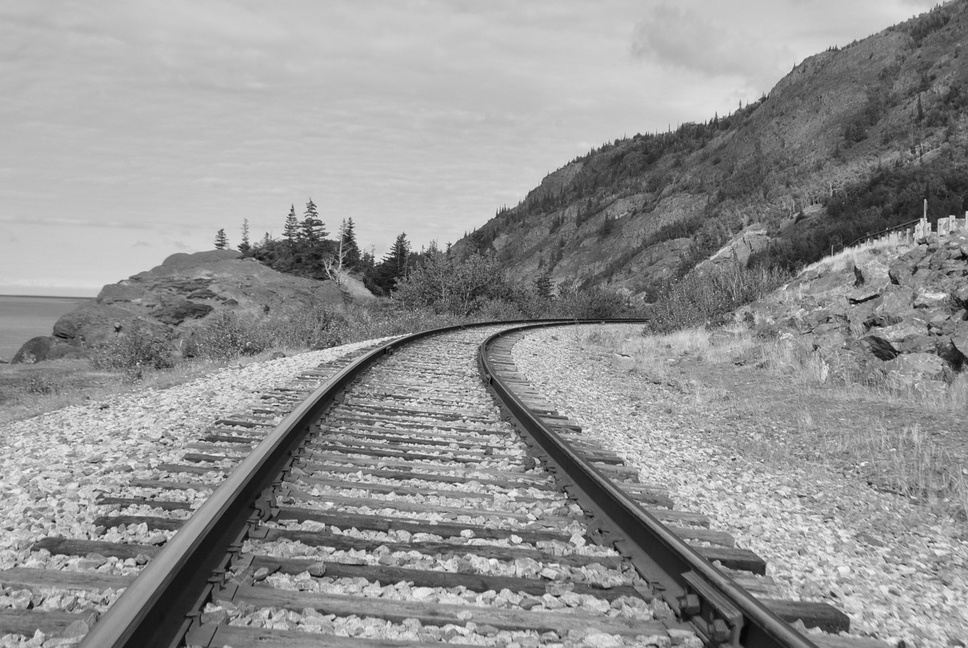
\includegraphics[width=0.45\textwidth]{src.jpg}
        \caption{Figura original}
        \label{fig:src}
\end{figure}

\begin{figure}[!ht]
    \centering
    \begin{subfigure}[ht]{0.45\textwidth}
        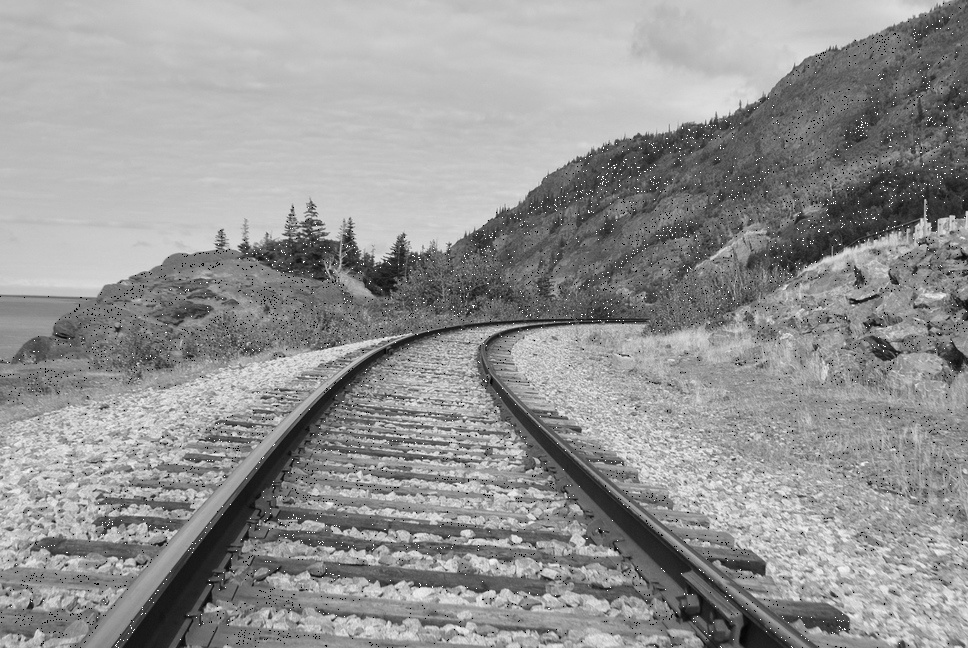
\includegraphics[width=\textwidth]{sp.jpg}
        \caption{Com ruído \textit{salt and pepper}}
    \end{subfigure}
    \qquad
    \begin{subfigure}[ht]{0.45\textwidth}
        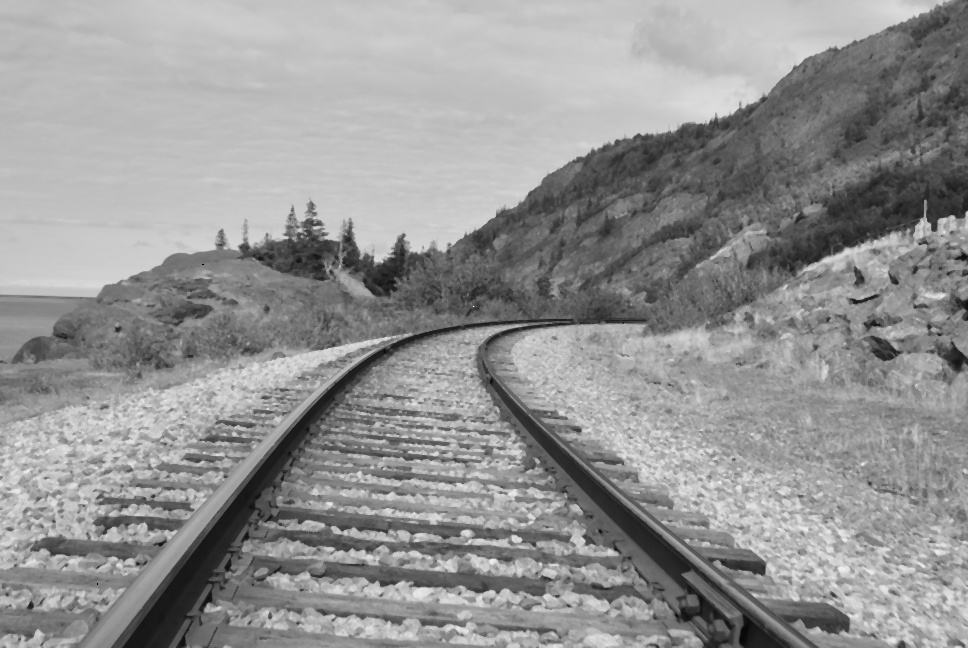
\includegraphics[width=\textwidth]{sp_median.jpg}
        \caption{Filtro da mediana em ruído \textit{salt and pepper}}
    \end{subfigure}
    \\
    \begin{subfigure}[ht]{0.45\textwidth}
        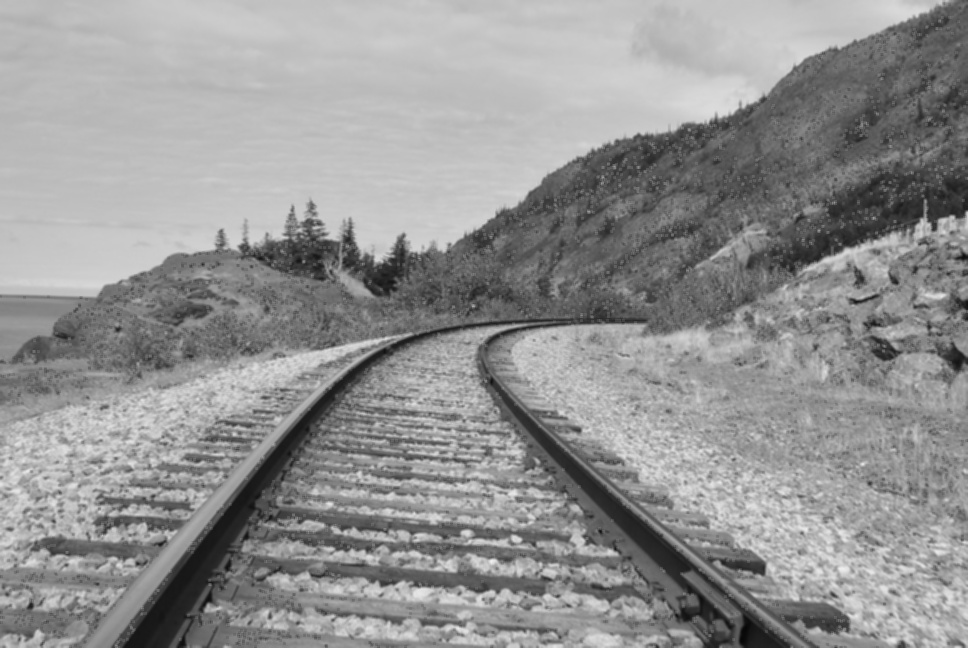
\includegraphics[width=\textwidth]{sp_gaussian.jpg}
        \caption{Filtro da Gaussiana em \textit{salt and pepper}}
    \end{subfigure}
    \qquad
    \begin{subfigure}[ht]{0.45\textwidth}
        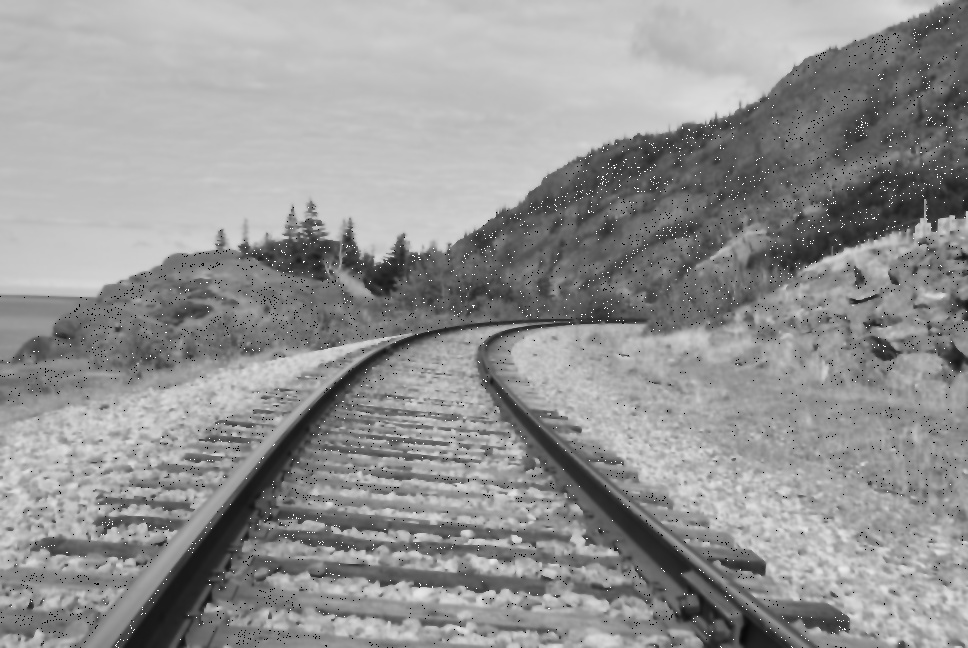
\includegraphics[width=\textwidth]{sp_aniso.jpg}
        \caption{Difusão anisotrópica em \textit{salt and pepper}}
    \end{subfigure}
    \\
    \begin{subfigure}[ht]{0.45\textwidth}
        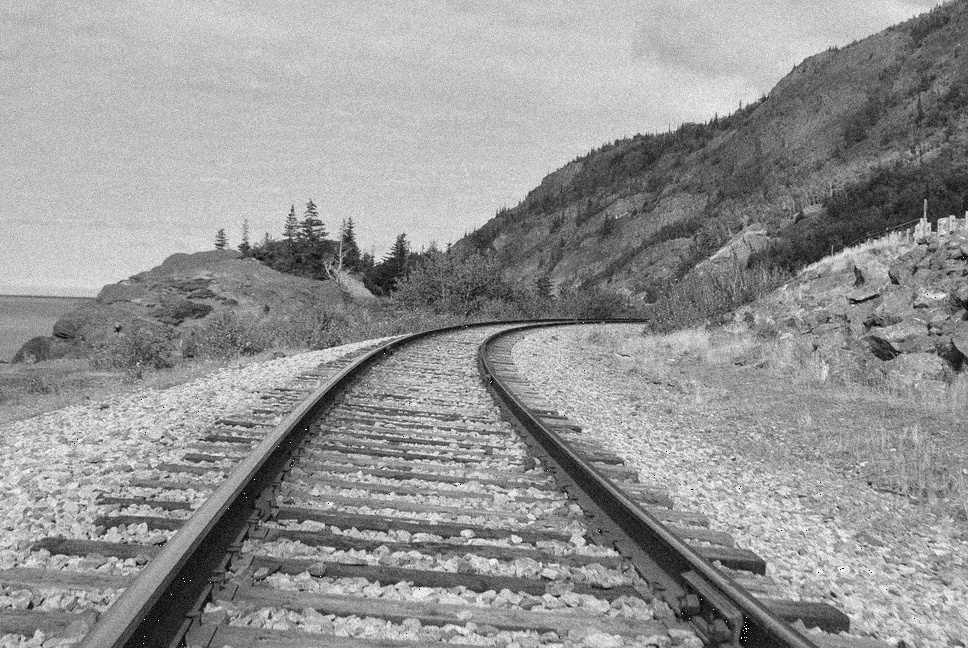
\includegraphics[width=\textwidth]{ga.jpg}
        \caption{Com ruído Gaussiano}
    \end{subfigure}
    \qquad
    \begin{subfigure}[ht]{0.45\textwidth}
        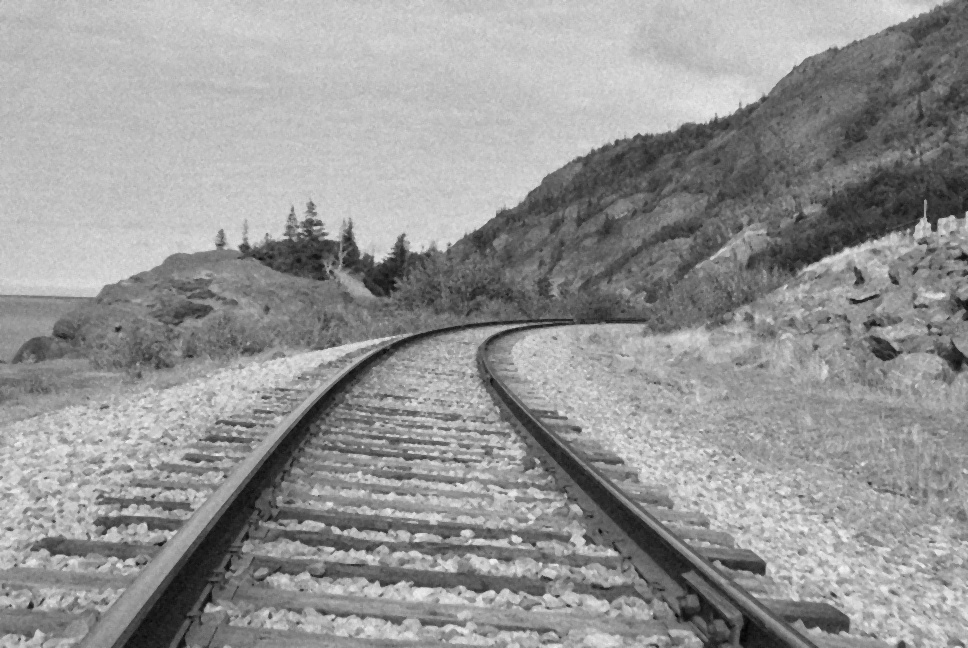
\includegraphics[width=\textwidth]{ga_median.jpg}
        \caption{Filtro da mediana em ruído Gaussiano}
    \end{subfigure}
    \\
    \begin{subfigure}[ht]{0.45\textwidth}
        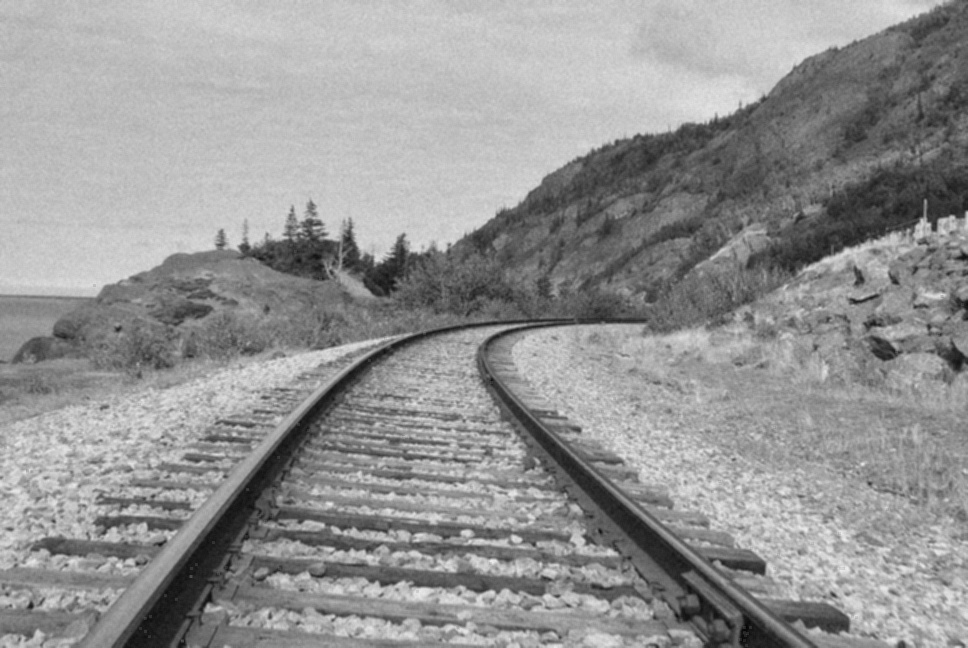
\includegraphics[width=\textwidth]{ga_gaussian.jpg}
        \caption{Filtro da Gaussiana em ruído Gaussiano}
    \end{subfigure}
    \qquad
    \begin{subfigure}[ht]{0.45\textwidth}
        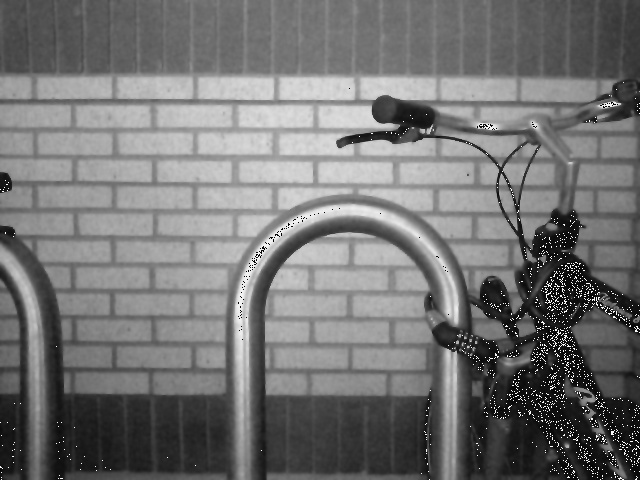
\includegraphics[width=\textwidth]{ga_aniso.jpg}
        \caption{Difusão anisotrópica em ruído gaussiano}
    \end{subfigure}
    \caption{Imagens com ruídos e com filtros aplicados}
    \label{fig:all}
\end{figure}

\begin{table}[!ht]
\begin{tabular}{cccccc}
\toprule
Filtro & Ruído & Total & Médio quadrático & Sinal Ruído & SSIM \\ \midrule
\multirow{2}{*}{Gaussiano}              & Gaussiano         & 78489 & 0.505 & 1.019 & 0.967 \\
                                        & Sal e pimenta     & 84155 & 0.523 & 0.963 & 0.983 \\\midrule
\multirow{2}{*}{Mediana}                & Gaussiano         & 84850 & 0.526 & 0.976 & 0.985 \\
                                        & Sal e pimenta    & 84832 & 0.525 & 0.947 & 0.995 \\\midrule
\multirow{2}{*}{Difusão anisotrópica}   & Gaussiano     & 170205517 & 23.538 & 29.630 & 0.913 \\
                                        & Sal e pimenta & 107418886 & 18.699 & 45.079 & 0.945 \\\bottomrule
\end{tabular}
\caption{Medidas de erros e similaridade para as images da Figura \ref{fig:all}}
\label{tab:results}
\end{table}

Como podemos ver na Tabela \ref{tab:results}, todos os índices são compatíveis entre si. Isto é, imagens que tiveram alto erro total, erro médio quadrático ou sinal-ruído tiveram os menores valores de $\mathit{SSIM}$. Curiosamente, a Difusão anisotrópica foi a que apresentou os piores resultados, tanto visualmente como pelos índices.

\subsection{Difusão anisotrópica e o $\mathit{SSIM}$}
Para a difusão anisotrópica, estudou-se como a variação dos parâmetros número de iterações, $\kappa$ e $\gamma$ afetava a imagem original, através de um \textit{grid search}. Os resultados do índice de similaridade estrutural para cada item foram plotados nos gráficos da Figura \ref{fig:simm_aniso}. Podemos ver como o número de iterações claramente borra a imagem, já que o $\mathit{SSIM}$ decresce conforme aumentamos o número de iterações. O mesmo pode ser dito para $\gamma$. Aumentar $\kappa$, por outro lado, tem o efeito inverso - a imagem produzida é mais parecida com a original, o que pode ser constatado com o maior valor de $\mathit{SSIM}$.

\begin{figure}[!htb]
\begin{subfigure}[ht]{0.45\columnwidth}
\begin{tikzpicture}
    \begin{axis}[xlabel=Iterações, ylabel=SSIM]
    \addplot coordinates {
( 1 , 0.915177942542 )
( 51 , 0.886941784946 )
( 101 , 0.866595195783 )
( 151 , 0.851691418409 )
( 201 , 0.83953047326 )
( 251 , 0.8293627615 )
( 301 , 0.820514897407 )
( 351 , 0.812721788225 )
( 401 , 0.805870831974 )
( 451 , 0.79974339225 )};
    \end{axis}
\end{tikzpicture}
\caption{Variação do número de interações}
\end{subfigure}
\qquad
\begin{subfigure}[ht]{0.45\columnwidth}
\begin{tikzpicture}
    \begin{axis}[xlabel=$\kappa$, ylabel=SSIM]
    \addplot coordinates {
( 1 , 0.909192998739 )
( 51 , 0.912909821173 )
( 101 , 0.911403807952 )
( 151 , 0.9599412168 )
( 201 , 0.965680017742 )
( 251 , 0.966272814367 )
( 301 , 0.966464712277 )
( 351 , 0.966560333193 )
( 401 , 0.966614383602 )
( 451 , 0.966649017241 )};
    \end{axis}
\end{tikzpicture}
\caption{Variação de $\kappa$.}
\end{subfigure}
\\
\begin{subfigure}[ht]{0.45\columnwidth}
\begin{tikzpicture}
    \begin{axis}[xlabel=$\gamma$, ylabel=SSIM]
    \addplot coordinates {
( 0.002 , 0.91067806574 )
( 0.102 , 0.912886329381 )
( 0.202 , 0.904948974613 )
( 0.302 , 0.892062808193 )
( 0.402 , 0.868458974177 )
( 0.502 , 0.85516485332 )
( 0.602 , 0.843687861726 )
( 0.702 , 0.834978764209 )
( 0.802 , 0.824419203523 )
( 0.902 , 0.810539185831 )};
    \end{axis}
\end{tikzpicture}
\caption{Variação de $\gamma$}
\end{subfigure}
\caption{Variação do SSIM de acordo com alterações nos parâmetros da difusão anisotrópica.}
\label{fig:simm_aniso}
\end{figure}

\begin{thebibliography}{99}
    \bibitem{article} WANG, Z.; BOVIK, Alan C.;SHEIKH, Hamid R.; SIMONCELLI, Eero P.; \textbf{Image Quality Assessment: From error visibility to structural similarity}. IEEE Transactions on Image Processing, vol. 13, no. 4, 2004.
\end{thebibliography}

\end{document}
